\chapter{Keelektronegatifan, Kepolaran, dan Gaya Antarmolekul}\label{ch:g11:polarity-and-cohesion}

Seekor tokek berlari menaiki kaca jendela dan bergantung di kaca itu
hanya dengan satu jari kaki, tanpa lem dan tanpa alat pengisap. \omterm{def:g7:atoms-and-molecules:molecule}{Molekul}
air, \ce{H2O}, lebih ringan daripada \omterm{def:g7:atoms-and-molecules:molecule}{molekul} hidrogen sulfida, \ce{H2S},
tetapi air mendidih pada \qty{100}{\celsius} sedangkan hidrogen sulfida
tetap berupa gas sampai \qty{-60}{\celsius}. Kedua kisah itu tentang hal
yang sama: gaya yang mengikat \omterm{def:g7:atoms-and-molecules:molecule}{molekul} satu sama lain, dan dengan benda
lain. Gaya itu jauh lebih lemah daripada \omterm{def:g10:lewis-and-shape:covalent-bond}{ikatan kovalen} di dalam
\omterm{def:g7:atoms-and-molecules:molecule}{molekul}, tetapi gaya itulah yang menentukan apakah sebuah zat berupa
gas, cairan, atau padatan pada suhu kamar, dan apakah seekor tokek
jatuh.

\begin{recall}
\omterm{def:g10:lewis-and-shape:covalent-bond}{Ikatan kovalen} adalah sepasang \omterm{def:g9:inside-the-atom:nucleus}{elektron} yang digunakan bersama oleh dua
\omterm{def:g7:atoms-and-molecules:atom}{atom}; \omterm{def:g10:lewis-and-shape:lewis-structure}{struktur Lewis} memperlihatkan \omterm{def:g10:lewis-and-shape:lone-pair}{pasangan elektron ikatan} dan
\omterm{def:g10:lewis-and-shape:lone-pair}{pasangan elektron bebas}, dan pasangan-pasangan di sekeliling \omterm{def:g7:atoms-and-molecules:atom}{atom} pusat
menentukan bentuk \omterm{def:g7:atoms-and-molecules:molecule}{molekul} (\cref{ch:g10:lewis-and-shape}). \omterm{def:g9:ions:ion}{Ion}
bermuatan; dalam padatan \omterm{def:g9:ions:ion}{ion}, \omterm{def:g9:ions:ion}{ion} positif dan \omterm{def:g9:ions:ion}{ion} negatif saling tarik
(\cref{ch:g9:ions}).
\end{recall}

\begin{omfigure}
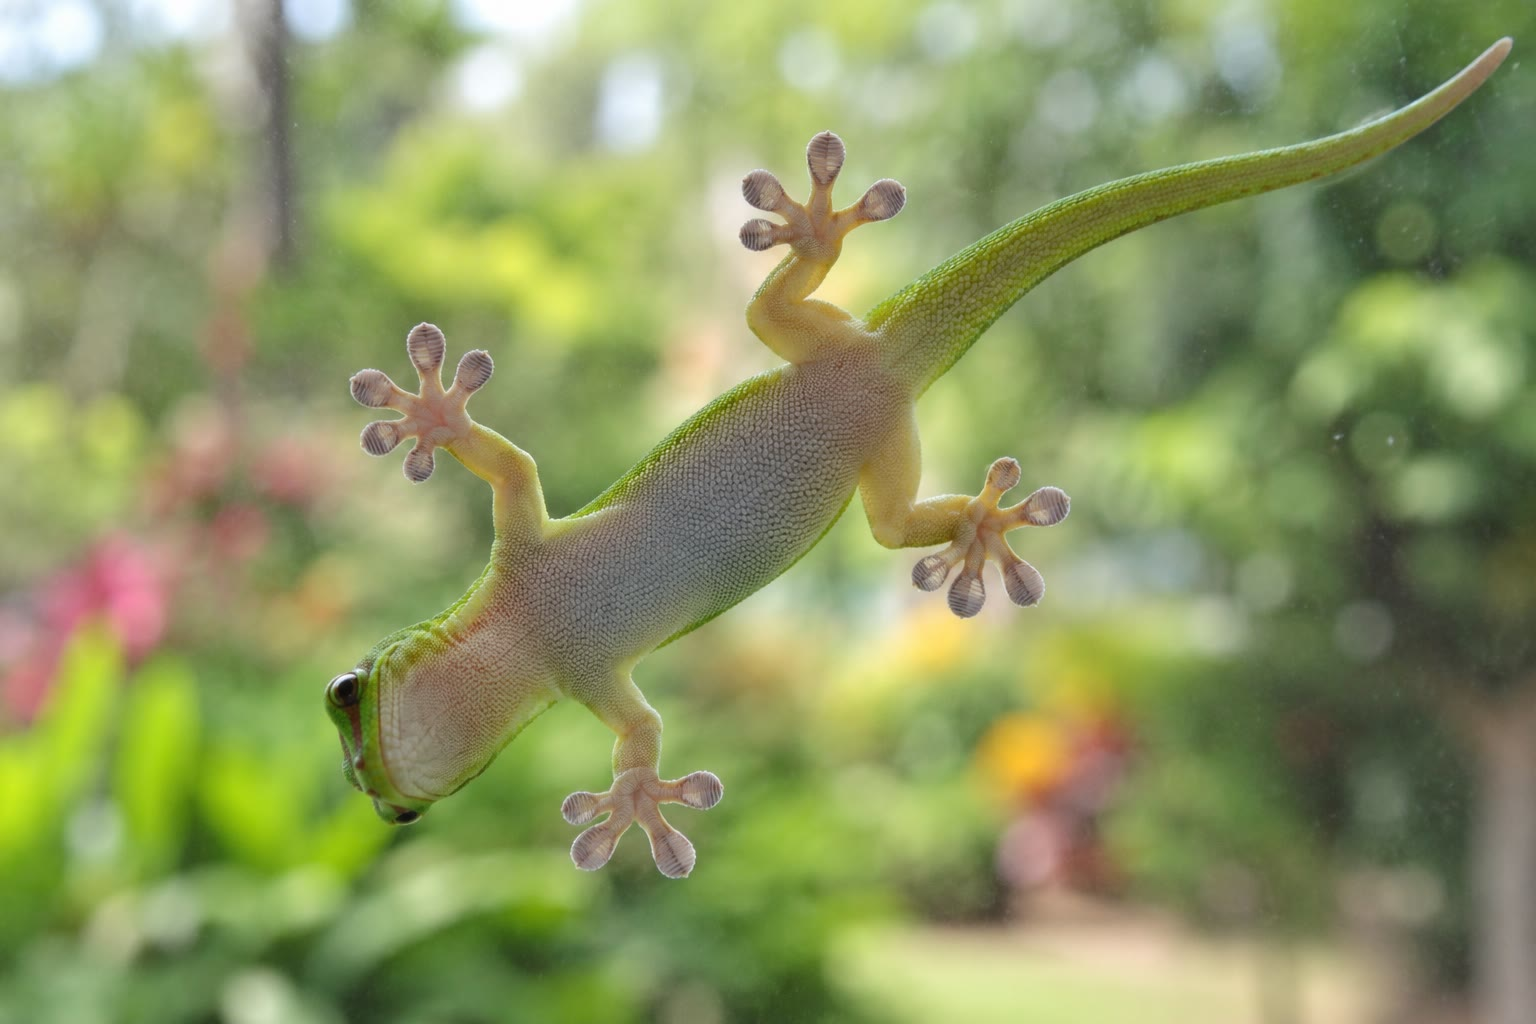
\includegraphics[width=0.5\linewidth]{images/book1/ai/g11-gecko-glass.jpg}

{\small Seekor tokek di atas kaca: bantalan jari kakinya menempel karena
gaya antarmolekul.}
\end{omfigure}

\section{Keelektronegatifan}

\begin{definition}[Keelektronegatifan]\label{def:g11:polarity-and-cohesion:electronegativity}
Yang disebut \emph{keelektronegatifan}\index{keelektronegatifan} sebuah
unsur mengukur seberapa kuat \omterm{def:g7:atoms-and-molecules:atom}{atom-atomnya}, dalam sebuah \omterm{def:g7:atoms-and-molecules:molecule}{molekul},
menarik \omterm{def:g9:inside-the-atom:nucleus}{elektron-elektron} ikatan yang digunakan bersama. Keelektronegatifan
adalah bilangan tanpa satuan; pada skala yang lazim nilainya berkisar
dari sekitar 0.8 sampai sekitar 4.
\end{definition}

\begin{omfigure}
% ledger: en:H, en:Li, en:Be, en:B, en:C, en:N, en:O, en:F, en:Na, en:Mg, en:Al, en:Si, en:P, en:S, en:Cl, en:K, en:Ca
\omperiodictable[upto=20, f block=false, cell=0.9cm, values={H/2.20,
  Li/0.98, Be/1.57, B/2.04, C/2.55, N/3.04, O/3.44, F/3.98, Na/0.93,
  Mg/1.31, Al/1.61, Si/1.90, P/2.19, S/2.58, Cl/3.16, K/0.82, Ca/1.00},
  highlight={F,O,N,Cl}]

{\small \omterm{def:g11:polarity-and-cohesion:electronegativity}{Keelektronegatifan} dua puluh unsur pertama (skala Pauling;
tidak ada nilai untuk helium, neon, dan argon, yang di sini tidak
membentuk ikatan). Disorot: keempat unsur yang paling elektronegatif.}
\end{omfigure}

\begin{proposition}[Kecenderungan dalam tabel]\label{prop:g11:polarity-and-cohesion:trends}
% ledger: en:F, en:Li, en:Cl, en:K
\omterm{def:g11:polarity-and-cohesion:electronegativity}{Keelektronegatifan} meningkat dari kiri ke kanan sepanjang periode dan
menurun dari atas ke bawah dalam \omterm{def:g9:periodic-table-first-look:period}{golongan}. Fluorin (3.98) adalah unsur
yang paling elektronegatif; \omterm{def:g10:electron-shells:family}{logam alkali} adalah yang paling kurang
(litium 0.98, kalium 0.82).
\end{proposition}

\begin{proof}
Dibaca pada tabel: sepanjang periode 2, $0.98 < 1.57 < 2.04 < 2.55 < 3.04 <
3.44 < 3.98$; ke bawah \omterm{def:g9:periodic-table-first-look:period}{golongan} 17, fluorin $3.98$ berada di atas klorin
$3.16$; ke bawah \omterm{def:g9:periodic-table-first-look:period}{golongan} 1, $2.20$, $0.98$, $0.93$, $0.82$. (Mengapa
demikian dijelaskan dalam buku Tahun Pertama universitas.)
\end{proof}

\begin{history}[Skala Pauling, 1932]
Ahli kimia Linus Pauling menyusun skala \omterm{def:g11:polarity-and-cohesion:electronegativity}{keelektronegatifan} yang pertama
pada tahun 1932, dari energi ikatan antara \omterm{def:g7:atoms-and-molecules:atom}{atom-atom} yang berbeda. Ia
memberi fluorin nilai terbesar, dan skala yang dipakai dalam bab ini
masih dinamai menurut namanya.
\end{history}

\section{Ikatan polar dan molekul polar}

\begin{definition}[Ikatan polar, muatan parsial]\label{def:g11:polarity-and-cohesion:polar-bond}
\omterm{def:g10:lewis-and-shape:covalent-bond}{Ikatan kovalen} antara dua \omterm{def:g7:atoms-and-molecules:atom}{atom} yang \omterm{def:g11:polarity-and-cohesion:electronegativity}{keelektronegatifannya} berbeda
disebut \emph{ikatan polar}\index{ikatan polar}: pasangan bersamanya
berada lebih dekat ke \omterm{def:g7:atoms-and-molecules:atom}{atom} yang lebih elektronegatif. \omterm{def:g7:atoms-and-molecules:atom}{Atom} itu membawa
\emph{muatan parsial}\index{muatan parsial} negatif yang kecil, ditulis
$\delta^-$, dan \omterm{def:g7:atoms-and-molecules:atom}{atom} yang lain muatan parsial positif yang sama besar,
$\delta^+$.
\end{definition}

\begin{proposition}[Kapan sebuah ikatan polar?]\label{prop:g11:polarity-and-cohesion:polar-bond}
% ledger: en:C, en:H, en:O, en:Na, en:Cl
Ikatan antara dua \omterm{def:g7:atoms-and-molecules:atom}{atom} yang sama tidak polar. Antara \omterm{def:g7:atoms-and-molecules:atom}{atom-atom} yang
berbeda, makin besar selisih \omterm{def:g11:polarity-and-cohesion:electronegativity}{keelektronegatifannya}, makin polar
ikatannya; sebagai pegangan praktis, selisih di bawah sekitar 0.4
(seperti \ce{C-H}, $2.55 - 2.20 = 0.35$) dianggap nonpolar. Jika
selisihnya sangat besar (seperti Na dan Cl, $3.16 - 0.93 = 2.23$),
\omterm{def:g9:inside-the-atom:nucleus}{elektron-elektronnya} tidak digunakan bersama tetapi dipindahkan:
senyawanya \omterm{def:g9:ions:ionic-compound}{senyawa ion}.
\end{proposition}

\begin{proof}
Diterima tanpa bukti: hal ini mengikuti dari definisi \omterm{def:g11:polarity-and-cohesion:electronegativity}{keelektronegatifan},
sedangkan ambang-ambangnya merupakan kesepakatan.
\end{proof}

\begin{definition}[Molekul polar dan nonpolar]\label{def:g11:polarity-and-cohesion:polar-molecule}
Sebuah \omterm{def:g7:atoms-and-molecules:molecule}{molekul} disebut \emph{molekul polar}\index{molekul polar} jika
pusat muatan-muatan parsial positifnya dan pusat muatan-muatan parsial
negatifnya tidak berimpit; jika keduanya berimpit, \omterm{def:g7:atoms-and-molecules:molecule}{molekul} itu disebut
\emph{molekul nonpolar}\index{molekul nonpolar}.
\end{definition}

\begin{method}[Polarkah sebuah molekul?]\label{met:g11:polarity-and-cohesion:polar}
\begin{enumerate}
  \item Gambarlah \omterm{def:g10:lewis-and-shape:lewis-structure}{struktur Lewis} dan tentukan bentuk \omterm{def:g7:atoms-and-molecules:molecule}{molekulnya}.
  \item Tandai ikatan-ikatan polar dengan $\delta^+$ dan $\delta^-$.
  \item Jika tidak ada \omterm{def:g11:polarity-and-cohesion:polar-bond}{ikatan polar}, \omterm{def:g7:atoms-and-molecules:molecule}{molekulnya} nonpolar. Jika ada,
        perhatikan bentuknya: jika ikatan-ikatan polar itu tersusun
        simetris di sekeliling pusat, pengaruhnya saling meniadakan dan
        \omterm{def:g7:atoms-and-molecules:molecule}{molekulnya} nonpolar; jika tidak, \omterm{def:g7:atoms-and-molecules:molecule}{molekulnya} polar.
\end{enumerate}
\end{method}

\begin{omfigure}
\begin{tikzpicture}[font=\small]
  % water
  \begin{scope}
    \node[aO] (o) at (0,0) {};
    \node[aH] (h1) at (-0.82,-0.6) {};
    \node[aH] (h2) at (0.82,-0.6) {};
    \begin{scope}[on background layer]
      \draw[bond] (o.center) -- (h1.center); \draw[bond] (o.center) -- (h2.center);
    \end{scope}
    \node[omThm] at (0,0.55) {$2\delta^-$};
    \node[omDef] at (-1.22,-0.5) {$\delta^+$};
    \node[omDef] at (1.22,-0.5) {$\delta^+$};
    \fill[omDef] (0,-0.6) circle (0.06);
    \fill[omThm] (0,0) circle (0.06);
    \draw[densely dotted, black!60] (-0.82,-0.6) -- (0.82,-0.6);
    \draw[<-, black!60] (0.08,-0.64) -- (1.55,-1.05) node[right, align=left,
      font=\footnotesize] {pusat\\ $\delta^+$};
    \node[align=center, anchor=north] at (0,-1.8) {air: bengkok, \textbf{polar}};
  \end{scope}
  % carbon dioxide
  \begin{scope}[xshift=6cm]
    \node[aO] (o1) at (-1.15,0) {};
    \node[aC] (c) at (0,0) {};
    \node[aO] (o2) at (1.15,0) {};
    \begin{scope}[on background layer]
      \draw[bond, double, double distance=1.6pt] (o1.center) -- (c.center);
      \draw[bond, double, double distance=1.6pt] (c.center) -- (o2.center);
    \end{scope}
    \node[omThm] at (-1.15,0.55) {$\delta^-$};
    \node[omThm] at (1.15,0.55) {$\delta^-$};
    \node[omDef] at (0,0.55) {$2\delta^+$};
    \draw[->, omProp, thick] (-0.25,-0.45) -- (-1.0,-0.45);
    \draw[->, omProp, thick] (0.25,-0.45) -- (1.0,-0.45);
    \node[align=center, anchor=north] at (0,-1.8) {karbon dioksida: linear,\\
      \textbf{nonpolar}};
  \end{scope}
\end{tikzpicture}

{\small Pada air, bentuk yang bengkok menempatkan pusat \omterm{def:g11:polarity-and-cohesion:polar-bond}{muatan parsial}
positif (di antara \omterm{def:g7:atoms-and-molecules:atom}{atom-atom} hidrogen) di bawah \omterm{def:g7:atoms-and-molecules:atom}{atom} oksigen: \omterm{def:g7:atoms-and-molecules:molecule}{molekulnya}
polar. Pada karbon dioksida, kedua \omterm{def:g11:polarity-and-cohesion:polar-bond}{ikatan polar} menarik ke arah yang
berlawanan (anak panah) dan saling meniadakan: pusat-pusat muatannya
berimpit pada \omterm{def:g7:atoms-and-molecules:atom}{atom} karbon.}
\end{omfigure}


\begin{example}[Empat molekul]\label{ex:g11:polarity-and-cohesion:four}
Hidrogen klorida \ce{HCl} memiliki satu \omterm{def:g11:polarity-and-cohesion:polar-bond}{ikatan polar} dan bersifat polar,
klorin $\delta^-$. Amonia \ce{NH3}, sebuah piramida dengan tiga ikatan
\ce{N-H} yang polar, bersifat polar, nitrogen $\delta^-$. Metana
\ce{CH4} hanya memiliki ikatan \ce{C-H} yang hampir nonpolar: nonpolar.
Tetraklorometana \ce{CCl4} memiliki empat ikatan \ce{C-Cl} yang polar,
tetapi di sudut-sudut tetrahedron beraturan: pengaruhnya saling
meniadakan dan \omterm{def:g7:atoms-and-molecules:molecule}{molekulnya} nonpolar.
\end{example}

\section{Interaksi van der Waals}

\begin{definition}[Interaksi van der Waals]\label{def:g11:polarity-and-cohesion:van-der-waals}
Yang disebut \emph{interaksi van der Waals}\index{interaksi van der Waals}
adalah tarikan lemah antara \omterm{def:g7:atoms-and-molecules:molecule}{molekul-molekul} yang bertetangga, yang ada
di antara semua \omterm{def:g7:atoms-and-molecules:molecule}{molekul}, polar maupun tidak: \omterm{def:g9:inside-the-atom:nucleus}{elektron-elektron} setiap
\omterm{def:g7:atoms-and-molecules:molecule}{molekul} terus bergerak, dan muatan-muatan sesaat yang tidak merata pada
satu \omterm{def:g7:atoms-and-molecules:molecule}{molekul} menarik muatan-muatan \omterm{def:g7:atoms-and-molecules:molecule}{molekul} tetangganya. Di antara
\omterm{def:g7:atoms-and-molecules:molecule}{molekul-molekul} polar, \omterm{def:g11:polarity-and-cohesion:polar-bond}{muatan parsial} yang tetap menambahkan tarikan
lagi.
\end{definition}


\begin{proposition}[Molekul yang lebih besar lebih kuat menarik]\label{prop:g11:polarity-and-cohesion:size}
\omterm{def:g11:polarity-and-cohesion:van-der-waals}{Interaksi van der Waals} makin kuat seiring ukuran \omterm{def:g7:atoms-and-molecules:molecule}{molekul}, yaitu seiring
banyaknya \omterm{def:g9:inside-the-atom:nucleus}{elektron}; di antara \omterm{def:g7:atoms-and-molecules:molecule}{molekul-molekul} yang serupa, yang lebih
besar memiliki suhu leleh dan suhu didih yang lebih tinggi.
\end{proposition}

\begin{proof}
Diterima tanpa bukti: awan \omterm{def:g9:inside-the-atom:nucleus}{elektron} yang lebih besar lebih mudah
berubah bentuk, sehingga muatan-muatan sesaatnya lebih besar, dan
bidang sentuhnya dengan tetangga-tetangganya lebih luas.
\end{proof}

\begin{example}[Halogen]\label{ex:g11:polarity-and-cohesion:halogens}
% ledger: bp:F2, bp:Cl2, bp:Br2, bp:I2 (K values converted)
\omterm{def:g7:atoms-and-molecules:molecule}{Molekul-molekul} \ce{F2}, \ce{Cl2}, \ce{Br2}, \ce{I2} semuanya nonpolar
dan makin lama makin besar. Suhu didihnya naik bersamanya:
\qty{-188}{\celsius}, \qty{-34}{\celsius}, \qty{59}{\celsius}, dan
\qty{184}{\celsius}. Pada suhu kamar, fluorin dan klorin berupa gas,
bromin cairan, iodin padatan.
\end{example}

\begin{remark}[Tokek]\label{rem:g11:polarity-and-cohesion:gecko}
Satu \omterm{def:g11:polarity-and-cohesion:van-der-waals}{interaksi van der Waals} saja sangat kecil, tetapi interaksi-interaksi
itu saling menjumlah. Bantalan jari kaki tokek tertutup karpet rapat
rambut-rambut mikroskopis, yang masing-masing terbelah lagi menjadi
ujung-ujung yang lebih halus, yang cukup dekat dengan kaca sehingga
\omterm{def:g11:polarity-and-cohesion:van-der-waals}{interaksi van der Waals} bekerja pada luas total yang sangat besar.
\end{remark}

\section{Ikatan hidrogen}

\begin{definition}[Ikatan hidrogen]\label{def:g11:polarity-and-cohesion:hydrogen-bond}
Yang disebut \emph{ikatan hidrogen}\index{ikatan hidrogen} adalah tarikan
antara \omterm{def:g7:atoms-and-molecules:atom}{atom} hidrogen yang terikat pada \omterm{def:g7:atoms-and-molecules:atom}{atom} yang sangat elektronegatif
(nitrogen, oksigen, atau fluorin), yang membawa $\delta^+$ yang nyata,
dan \omterm{def:g10:lewis-and-shape:lone-pair}{pasangan elektron bebas} milik \omterm{def:g7:atoms-and-molecules:atom}{atom} nitrogen, oksigen, atau fluorin
yang lain, sering pada \omterm{def:g7:atoms-and-molecules:molecule}{molekul} tetangganya. Ikatan ini digambar sebagai
garis putus-putus, dan ketiga \omterm{def:g7:atoms-and-molecules:atom}{atom} yang terlibat hampir segaris.
\end{definition}

\begin{omfigure}
\begin{tikzpicture}[font=\small]
  % central water molecule and four neighbours, H-bonds dashed
  \newcommand{\water}[4]{% name, x, y, rotation
    \begin{scope}[shift={(#2,#3)}, rotate=#4]
      \node[aO] (#1o) at (0,0) {};
      \node[aH] (#1a) at (-0.6,-0.45) {};
      \node[aH] (#1b) at (0.6,-0.45) {};
    \end{scope}
    \begin{scope}[on background layer]
      \draw[bond] (#1o.center) -- (#1a.center); \draw[bond] (#1o.center) -- (#1b.center);
    \end{scope}}
  \water{m}{0}{0}{0}
  \water{p}{-1.62}{-1.215}{0}
  \water{q}{1.62}{-1.215}{0}
  \water{r}{-1.435}{1.435}{-8.13}
  \water{s}{1.435}{1.435}{8.13}
  % H-bonds: m's H to p's O and q's O; r's and s's H to m's O
  \draw[dashed, omDef, thick] (ma) -- (po);
  \draw[dashed, omDef, thick] (mb) -- (qo);
  \draw[dashed, omDef, thick] (rb) -- (mo);
  \draw[dashed, omDef, thick] (sa) -- (mo);
\end{tikzpicture}

{\small \omterm{def:g11:polarity-and-cohesion:hydrogen-bond}{Ikatan hidrogen} (putus-putus) di sekeliling sebuah \omterm{def:g7:atoms-and-molecules:molecule}{molekul} air
dalam air cair: kedua \omterm{def:g7:atoms-and-molecules:atom}{atom} hidrogennya berikatan dengan \omterm{def:g7:atoms-and-molecules:atom}{atom-atom} oksigen
dua \omterm{def:g7:atoms-and-molecules:molecule}{molekul} tetangga, dan kedua \omterm{def:g10:lewis-and-shape:lone-pair}{pasangan elektron bebas} \omterm{def:g7:atoms-and-molecules:atom}{atom} oksigennya
menerima \omterm{def:g7:atoms-and-molecules:atom}{atom-atom} hidrogen dua \omterm{def:g7:atoms-and-molecules:molecule}{molekul} lainnya.}
\end{omfigure}


\begin{example}[Etanol dan propana]\label{ex:g11:polarity-and-cohesion:ethanol}
% ledger: bp:C2H5OH, bp:C3H8 (K values converted)
\omterm{def:g7:atoms-and-molecules:molecule}{Molekul} etanol, \ce{CH3-CH2-OH} (\qty{46.0}{g/mol}), dan \omterm{def:g7:atoms-and-molecules:molecule}{molekul}
propana, \ce{CH3-CH2-CH3} (\qty{44.0}{g/mol}), hampir sama
ukurannya. Namun etanol mendidih pada \qty{78}{\celsius} dan propana
pada \qty{-42}{\celsius}. \omterm{def:g7:atoms-and-molecules:molecule}{Molekul-molekul} etanol, dengan gugus
\ce{O-H}-nya, membentuk \omterm{def:g11:polarity-and-cohesion:hydrogen-bond}{ikatan hidrogen} satu sama lain; \omterm{def:g7:atoms-and-molecules:molecule}{molekul-molekul}
propana tidak dapat.
\end{example}

\section{Kohesi padatan dan cairan}

\begin{definition}[Padatan molekul]\label{def:g11:polarity-and-cohesion:molecular-solid}
Yang disebut \emph{padatan molekul}\index{padatan molekul} adalah
padatan yang tersusun atas \omterm{def:g7:atoms-and-molecules:molecule}{molekul-molekul} yang terikat satu sama lain
oleh \omterm{def:g11:polarity-and-cohesion:van-der-waals}{interaksi van der Waals} dan, jika mungkin, \omterm{def:g11:polarity-and-cohesion:hydrogen-bond}{ikatan hidrogen}. Es,
iodin padat, dan gula adalah padatan \omterm{def:g7:atoms-and-molecules:molecule}{molekul}.
\end{definition}

\begin{proposition}[Kohesi dan perubahan wujud]\label{prop:g11:polarity-and-cohesion:cohesion}
Makin kuat tarikan antara partikel-partikel sebuah zat, makin tinggi
suhu leleh dan suhu didihnya. Menurut kekuatan yang makin besar:
\omterm{def:g11:polarity-and-cohesion:van-der-waals}{interaksi van der Waals}, \omterm{def:g11:polarity-and-cohesion:hydrogen-bond}{ikatan hidrogen}, dan tarikan antara \omterm{def:g9:ions:ion}{ion-ion}
dalam padatan \omterm{def:g9:ions:ion}{ion}.
\end{proposition}

\begin{proof}
Diterima tanpa bukti: meleleh dan mendidih menarik partikel-partikel
saling menjauh melawan tarikan-tarikan itu, yang memerlukan energi lebih
banyak, jadi suhu yang lebih tinggi, jika tarikan itu lebih kuat.
\end{proof}

\begin{example}[Tiga padatan]\label{ex:g11:polarity-and-cohesion:three}
% ledger: mp:NaCl, mp:water
Natrium klorida, sebuah padatan \omterm{def:g9:ions:ion}{ion}, meleleh pada \qty{801}{\celsius};
es, yang diikat oleh \omterm{def:g11:polarity-and-cohesion:hydrogen-bond}{ikatan hidrogen}, pada \qty{0}{\celsius}; metana
padat, yang hanya diikat oleh \omterm{def:g11:polarity-and-cohesion:van-der-waals}{interaksi van der Waals} antara \omterm{def:g7:atoms-and-molecules:molecule}{molekul-molekul}
kecil, jauh di bawah \qty{-150}{\celsius}.
\end{example}

\begin{omfigure}
\begin{tikzpicture}
\begin{axis}[width=0.6\linewidth, height=7cm, xmin=1.7, xmax=5.3,
    ymin=-190, ymax=120, xtick={2,3,4,5}, xlabel={periode},
    ylabel={suhu didih (\si{\celsius})}, axis lines*=left,
    ymajorgrids, grid style={gray!20}, tick label style={font=\small},
    label style={font=\small},
    legend style={font=\small, at={(1.02,0.5)}, anchor=west, draw=none},
    legend cell align=left]
  % ledger: bp:CH4, bp:SiH4, bp:GeH4, bp:NH3, bp:PH3, bp:AsH3, bp:SbH3, bp:H2O, bp:H2S, bp:H2Se, bp:HF, bp:HCl, bp:HBr, bp:HI (K values converted to degC)
  \addplot[thick, mark=*, black!70] coordinates {(2,-162.2) (3,-112) (4,-88.1)};
  \addplot[thick, mark=square*, omMeth] coordinates {(2,-33.4) (3,-87.8) (4,-62.5) (5,-18.4)};
  \addplot[thick, mark=triangle*, mark size=3pt, omThm] coordinates {(2,100.0) (3,-60.3) (4,-41.3)};
  \addplot[thick, mark=diamond*, mark size=3pt, omDef] coordinates {(2,19.6) (3,-85.1) (4,-66.4) (5,-35.1)};
  \legend{golongan 14 (\ce{CH4} \dots), golongan 15 (\ce{NH3} \dots),
    golongan 16 (\ce{H2O} \dots), golongan 17 (\ce{HF} \dots)}
  \node[font=\footnotesize, anchor=west] at (axis cs:2.05,100) {\ce{H2O}};
  \node[font=\footnotesize, anchor=west] at (axis cs:2.05,19.6) {\ce{HF}};
  \node[font=\footnotesize, anchor=west] at (axis cs:2.05,-33.4) {\ce{NH3}};
  \node[font=\footnotesize, anchor=north west] at (axis cs:2.05,-166) {\ce{CH4}};
\end{axis}
\end{tikzpicture}

{\small Suhu didih senyawa hidrogen dengan unsur-unsur \omterm{def:g9:periodic-table-first-look:period}{golongan} 14
sampai 17. Dalam setiap \omterm{def:g9:periodic-table-first-look:period}{golongan}, suhu didih naik seiring ukuran
\omterm{def:g7:atoms-and-molecules:molecule}{molekul}, kecuali anggota pertama \omterm{def:g9:periodic-table-first-look:period}{golongan} 15, 16, dan 17, yang terlalu
tinggi: amonia, air, dan hidrogen fluorida membentuk \omterm{def:g11:polarity-and-cohesion:hydrogen-bond}{ikatan hidrogen}.
(Tidak ada nilai yang digambar jika sumber yang dipakai tidak
memberikannya.)}
\end{omfigure}

\begin{remark}[Es dan salju]\label{rem:g11:polarity-and-cohesion:ice}
Dalam es, setiap \omterm{def:g7:atoms-and-molecules:molecule}{molekul} air berikatan hidrogen dengan empat
tetangganya, dalam jaringan terbuka berupa cincin-cincin segi enam.
Jaringan itu menyisakan lebih banyak ruang kosong daripada air cair,
tempat ikatan-ikatan itu terus putus dan terbentuk kembali: es lebih
kecil massa jenisnya daripada air dan terapung. Simetri lipat enam pada
kristal salju mencerminkan cincin-cincin segi enam jaringan itu.
\end{remark}

\begin{omfigure}
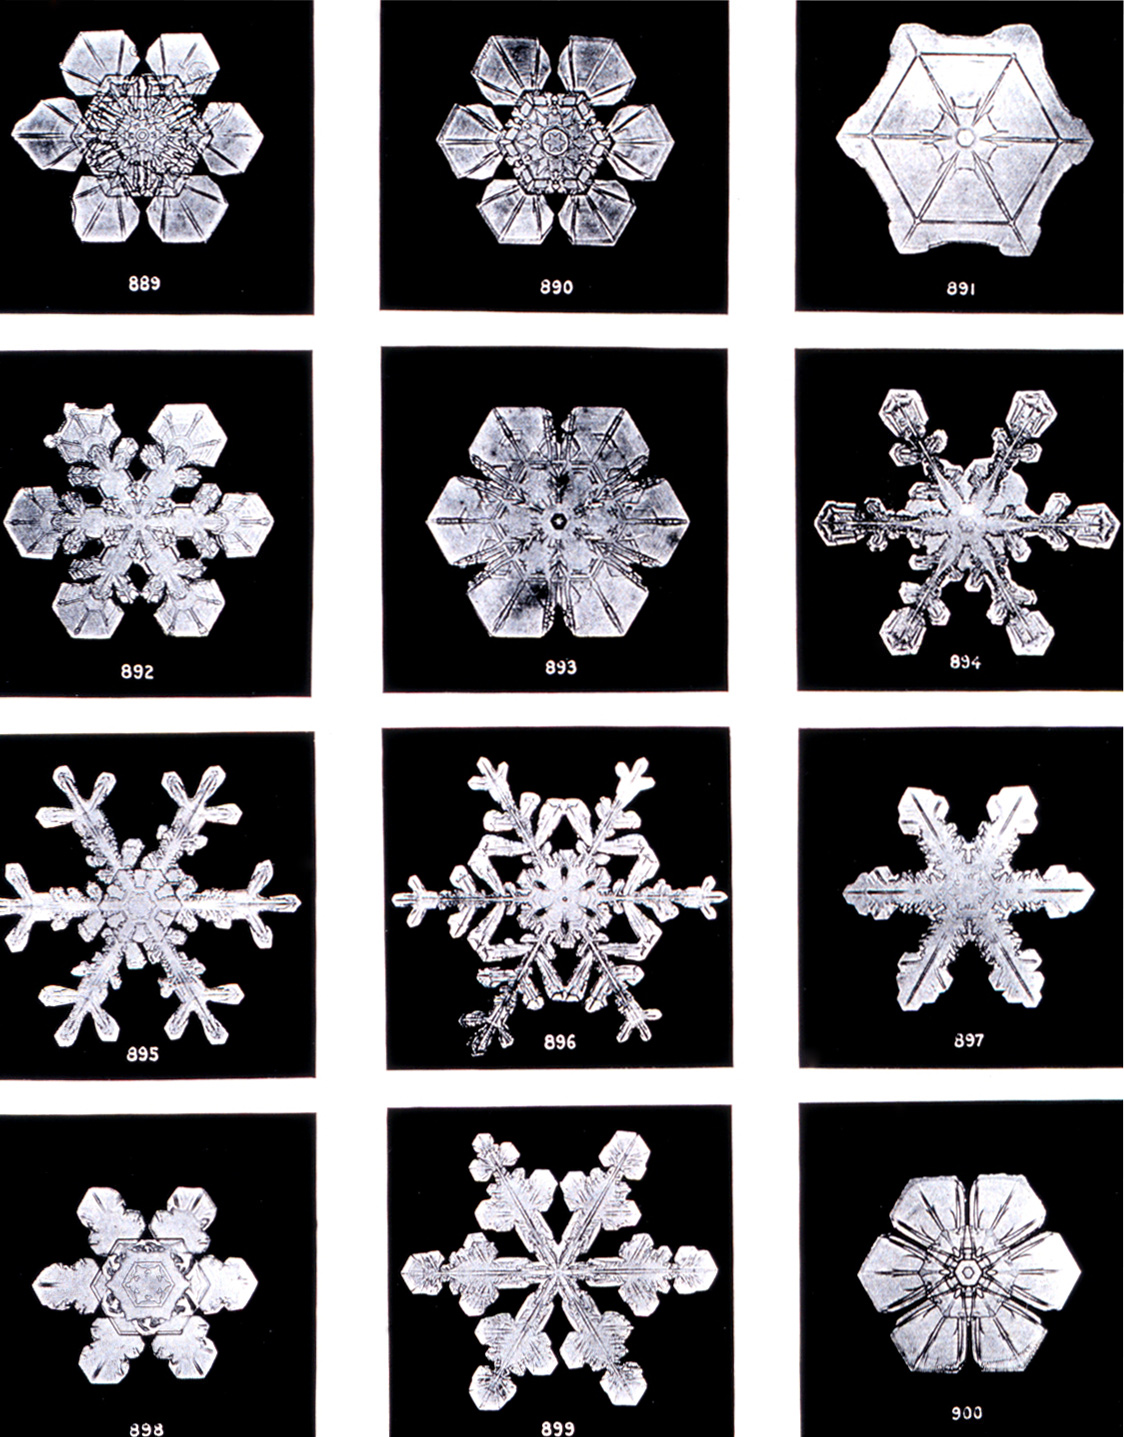
\includegraphics[width=0.36\linewidth]{images/book1/snowflakes.jpg}

{\small Kristal-kristal salju yang dipotret Wilson Bentley pada awal
tahun 1900-an: setiap kristal memiliki enam cabang.}
\end{omfigure}

\section{Latihan}


\begin{exercise}[$\star$]\label{exo:g11:polarity-and-cohesion:1}
Pada ikatan \ce{H-Cl}, \ce{O-H}, dan \ce{C-O}, \omterm{def:g7:atoms-and-molecules:atom}{atom} mana yang membawa
\omterm{def:g11:polarity-and-cohesion:polar-bond}{muatan parsial} $\delta^-$? Pakailah tabel \omterm{def:g11:polarity-and-cohesion:electronegativity}{keelektronegatifan}.
\end{exercise}

\begin{exercise}[$\star$]\label{exo:g11:polarity-and-cohesion:2}
Manakah di antara ikatan-ikatan berikut yang polar: \ce{H-H}, \ce{C-H},
\ce{O-H}, \ce{N-H}, \ce{Cl-Cl}, \ce{C-Cl}? Berikan selisih
\omterm{def:g11:polarity-and-cohesion:electronegativity}{keelektronegatifan} untuk masing-masing.
\end{exercise}

\begin{exercise}[$\star$]\label{exo:g11:polarity-and-cohesion:3}
Unsur mana yang lebih elektronegatif pada setiap pasangan: nitrogen atau
fosfor; oksigen atau belerang; karbon atau nitrogen; natrium atau
magnesium? Kecenderungan tabel yang mana yang diperlihatkan setiap
pasangan?
\end{exercise}

\begin{exercise}[$\star$]\label{exo:g11:polarity-and-cohesion:4}
Manakah di antara \ce{CH4}, \ce{NH3}, \ce{H2O}, dan \ce{HCl} yang dapat
membentuk \omterm{def:g11:polarity-and-cohesion:hydrogen-bond}{ikatan hidrogen} di antara \omterm{def:g7:atoms-and-molecules:molecule}{molekul-molekulnya} sendiri?
Jelaskan.
\end{exercise}

\begin{exercise}[$\star$]\label{exo:g11:polarity-and-cohesion:5}
Adakah tarikan antara \omterm{def:g7:atoms-and-molecules:molecule}{molekul-molekul} metana yang nonpolar? Mengapa
metana tetap berupa gas pada suhu kamar?
\end{exercise}

\begin{exercise}[$\star\star$]\label{exo:g11:polarity-and-cohesion:6}
Katakan apakah setiap \omterm{def:g7:atoms-and-molecules:molecule}{molekul} berikut polar: diklorometana \ce{CH2Cl2}
(tetrahedral), tetraklorometana \ce{CCl4}, amonia \ce{NH3}, karbon
dioksida \ce{CO2}, boron trifluorida \ce{BF3} (segitiga datar dengan
boron di tengahnya).
\end{exercise}

\begin{exercise}[$\star\star$]\label{exo:g11:polarity-and-cohesion:7}
Pada metanol, \ce{CH3-OH}, \omterm{def:g7:atoms-and-molecules:atom}{atom} hidrogen mana yang dapat diberikan dalam
\omterm{def:g11:polarity-and-cohesion:hydrogen-bond}{ikatan hidrogen}? \omterm{def:g7:atoms-and-molecules:atom}{Atom} mana yang dapat menerimanya? Dapatkah \omterm{def:g7:atoms-and-molecules:molecule}{molekul}
metanol dan \omterm{def:g7:atoms-and-molecules:molecule}{molekul} air membentuk \omterm{def:g11:polarity-and-cohesion:hydrogen-bond}{ikatan hidrogen} satu sama lain?
Gambarlah salah satunya.
\end{exercise}

\begin{exercise}[$\star\star$]\label{exo:g11:polarity-and-cohesion:8}
Jelaskan mengapa suhu didih naik menurut urutan \ce{CH4} <
\ce{SiH4} < \ce{GeH4}.
\end{exercise}

\begin{exercise}[$\star\star$]\label{exo:g11:polarity-and-cohesion:9}
Pada grafik suhu didih hidrida-hidrida itu, \omterm{def:g9:periodic-table-first-look:period}{golongan} mana yang tidak
memperlihatkan nilai yang tidak biasa pada anggota pertamanya? Mengapa?
\end{exercise}

\begin{exercise}[$\star\star$]\label{exo:g11:polarity-and-cohesion:10}
% ledger: en:H, en:Cl, en:Br, en:I, bp:HCl, bp:HBr, bp:HI
Ikatan \ce{H-Cl}, \ce{H-Br}, \ce{H-I} makin lama makin kurang polar
(\omterm{def:g11:polarity-and-cohesion:electronegativity}{keelektronegatifan} klorin, bromin, dan iodin adalah 3.16, 2.96, dan
2.66), tetapi suhu didihnya naik: \qty{-85}{\celsius},
\qty{-66}{\celsius}, \qty{-35}{\celsius}. Interaksi mana yang menang, dan
mengapa?
\end{exercise}

\begin{exercise}[$\star\star$]\label{exo:g11:polarity-and-cohesion:11}
Pada suhu kamar klorin berupa gas dan iodin padatan, padahal keduanya
tersusun atas \omterm{def:g7:atoms-and-molecules:molecule}{molekul-molekul} nonpolar \ce{X2}. Jelaskan.
\end{exercise}

\begin{exercise}[$\star\star\star$]\label{exo:g11:polarity-and-cohesion:12}
% ledger: bp:C2H5OH, bp:CH3OCH3, bp:C3H8
Etanol \ce{CH3-CH2-OH}, metoksimetana \ce{CH3-O-CH3}, dan propana
\ce{CH3-CH2-CH3} memiliki \omterm{def:g10:the-mole:molar-mass}{massa molar} yang hampir sama. Ketiganya
mendidih pada \qty{78}{\celsius}, \qty{-25}{\celsius}, dan
\qty{-42}{\celsius}. Manakah yang polar? Manakah yang membentuk \omterm{def:g11:polarity-and-cohesion:hydrogen-bond}{ikatan
hidrogen} di antara \omterm{def:g7:atoms-and-molecules:molecule}{molekul-molekulnya} sendiri? Jelaskan urutannya.
\end{exercise}

\begin{exercise}[$\star\star\star$]\label{exo:g11:polarity-and-cohesion:13}
Dalam es, setiap \omterm{def:g7:atoms-and-molecules:molecule}{molekul} air berikatan hidrogen dengan empat
tetangganya, dalam jaringan terbuka; dalam air cair, jaringan itu terus
putus dan sebagian runtuh. Jelaskan mengapa es terapung di atas air.
Mengapa hal ini penting bagi ikan di danau yang membeku?
\end{exercise}

\begin{exercise}[$\star\star\star$]\label{exo:g11:polarity-and-cohesion:14}
Urutkan menurut suhu leleh yang makin tinggi, dan berikan alasan dengan
tarikan antara partikel-partikelnya: kalium klorida \ce{KCl}, es
\ce{H2O}, metana padat \ce{CH4}.
\end{exercise}

\begin{exercise}[$\star\star\star$]\label{exo:g11:polarity-and-cohesion:15}
% ledger: en:F, en:O, bp:HF, bp:H2O
Fluorin lebih elektronegatif daripada oksigen, sehingga ikatan \ce{H-F}
lebih polar daripada ikatan \ce{O-H}. Namun air mendidih pada
\qty{100}{\celsius} dan hidrogen fluorida pada \qty{20}{\celsius}.
Hitunglah \omterm{def:g7:atoms-and-molecules:atom}{atom} hidrogen yang dapat diberikan setiap \omterm{def:g7:atoms-and-molecules:molecule}{molekul} dan \omterm{def:g10:lewis-and-shape:lone-pair}{pasangan
elektron bebas} yang dapat dipakainya untuk menerima, lalu jelaskan.
\end{exercise}

\section{Soal: Mengapa Air Mendidih pada \texorpdfstring{\qty{100}{\celsius}}{100 derajat Celsius}?}

\begin{problem}[{Soal akhir pekan --- tanpa ikatan hidrogen, pada suhu
berapa air akan mendidih?}]
\label{pb:g11:polarity-and-cohesion:1}
% ledger: en:H, en:O, en:S, en:Se, bp:H2O, bp:H2S, bp:H2Se, bp:CH4, bp:SiH4, bp:GeH4, bp:HCl, bp:HBr, bp:HF, bp:NH3, bp:PH3, bp:AsH3
Oksigen, belerang, dan selenium berada dalam \omterm{def:g9:periodic-table-first-look:period}{golongan} yang sama dalam
tabel, dan ketiganya membentuk senyawa dengan hidrogen: \ce{H2O},
\ce{H2S}, \ce{H2Se}. Dalam setiap \omterm{def:g9:periodic-table-first-look:period}{golongan} hidrida, suhu didih biasanya
naik seiring ukuran \omterm{def:g7:atoms-and-molecules:molecule}{molekul}. Air melanggar aturan itu. Seberapa jauh?

\medskip
\noindent\textbf{Bagian I --- Tiga \omterm{def:g7:atoms-and-molecules:molecule}{molekul}.}
\begin{enumerate}
  \item Gambarlah \omterm{def:g10:lewis-and-shape:lewis-structure}{struktur Lewis} \ce{H2O}, \ce{H2S}, dan \ce{H2Se}.
        Mengapa ketiganya mirip?
  \item Hitung \omterm{def:g10:the-mole:molar-mass}{massa molarnya}.
  \item Hitung selisih \omterm{def:g11:polarity-and-cohesion:electronegativity}{keelektronegatifan} ikatan \ce{O-H}, \ce{S-H}, dan
        \ce{Se-H} (oksigen 3.44, belerang 2.58, selenium 2.55, hidrogen
        2.20). Ikatan mana yang jelas polar?
  \item Bagaimana bentuk ketiga \omterm{def:g7:atoms-and-molecules:molecule}{molekul} itu? Apakah ketiganya polar?
  \item Hitung \omterm{def:g9:inside-the-atom:nucleus}{elektron} setiap \omterm{def:g7:atoms-and-molecules:molecule}{molekul}. \omterm{def:g7:atoms-and-molecules:molecule}{Molekul} mana yang memiliki
        \omterm{def:g11:polarity-and-cohesion:van-der-waals}{interaksi van der Waals} paling kuat?
\end{enumerate}

\medskip
\noindent\textbf{Bagian II --- \omterm{def:g11:polarity-and-cohesion:hydrogen-bond}{Ikatan hidrogen}.}
\begin{enumerate}[resume]
  \item Manakah di antara ketiga senyawa itu yang membentuk \omterm{def:g11:polarity-and-cohesion:hydrogen-bond}{ikatan
        hidrogen} di antara \omterm{def:g7:atoms-and-molecules:molecule}{molekul-molekulnya}? Mengapa yang lain tidak?
  \item Paling banyak dalam berapa \omterm{def:g11:polarity-and-cohesion:hydrogen-bond}{ikatan hidrogen} sebuah \omterm{def:g7:atoms-and-molecules:molecule}{molekul} air
        dapat ikut serta? Gambarlah.
  \item Interaksi apa yang mengikat \omterm{def:g7:atoms-and-molecules:molecule}{molekul-molekul} hidrogen sulfida dalam
        keadaan cair?
\end{enumerate}

\medskip
\noindent\textbf{Bagian III --- Kecenderungannya.}
\begin{enumerate}[resume]
  \item Hidrogen sulfida mendidih pada \qty{212.9}{K} dan hidrogen
        selenida pada \qty{-41.3}{\celsius}. Nyatakan yang pertama dalam
        derajat Celsius ($\theta = T - 273.15$).
  \item Berapa kenaikan suhu didih dari periode 3 (\ce{H2S}) ke periode 4
        (\ce{H2Se})?
  \item Mengapa suhu didih itu naik?
  \item Dengan menganggap kenaikan yang sama dari periode 2 ke periode 3,
        pada suhu berapa \ce{H2O} yang ``normal'' akan mendidih?
  \item Ujilah cara itu pada \omterm{def:g9:periodic-table-first-look:period}{golongan} 14: \ce{SiH4} mendidih pada
        \qty{-112}{\celsius} dan \ce{GeH4} pada \qty{-88.1}{\celsius}.
        Ramalkan suhu didih \ce{CH4}, lalu bandingkan dengan nilai
        sebenarnya, \qty{-162}{\celsius}. Apakah ekstrapolasinya tepat?
  \item Lakukan hal yang sama untuk \omterm{def:g9:periodic-table-first-look:period}{golongan} 17 (\ce{HCl}
        \qty{-85.1}{\celsius}, \ce{HBr} \qty{-66.4}{\celsius}), lalu
        bandingkan dengan \ce{HF}, \qty{19.6}{\celsius}.
\end{enumerate}

\medskip
\noindent\textbf{Bagian IV --- Selisihnya.}
\begin{enumerate}[resume]
  \item Air sebenarnya mendidih pada \qty{100}{\celsius}. Seberapa besar
        selisih antara nilai sebenarnya dan nilai hasil ekstrapolasi?
  \item Hal yang sama untuk amonia, dengan memakai \ce{PH3}
        \qty{-87.8}{\celsius} dan \ce{AsH3} \qty{-62.5}{\celsius}; amonia
        sebenarnya mendidih pada \qty{-33.4}{\celsius}.
  \item Urutkan air, hidrogen fluorida, dan amonia menurut besarnya
        selisih itu, lalu jelaskan urutan itu dengan menghitung \omterm{def:g11:polarity-and-cohesion:hydrogen-bond}{ikatan
        hidrogen}.
  \item Tanpa \omterm{def:g11:polarity-and-cohesion:hydrogen-bond}{ikatan hidrogen}, apakah air akan berupa padatan, cairan,
        atau gas pada suhu kamar? Apa artinya bagi Bumi?
  \item Mengapa jawaban soal 12 hanya sebuah perkiraan?
  \item Nyatakan jawaban akhirnya: kira-kira pada suhu berapa air akan
        mendidih tanpa \omterm{def:g11:polarity-and-cohesion:hydrogen-bond}{ikatan hidrogen}?
\end{enumerate}
\end{problem}
